% !TEX program = xelatex
% !Mode:: "Tex:UTF-8"

\documentclass[
        % handout, % print version
        % draft, % fast testing version
        ]{beamer}

% math
\usepackage{amssymb,latexsym,amssymb,amsmath,amsbsy,amsopn,amstext,upgreek}

% pictures, colors and multicolumn
\usepackage{color,multicol}
\usepackage{graphicx,wrapfig,fancybox,graphics}
\usepackage{picins}
\usepackage{pgf}
\usepackage{media9}

% pdf options
\usepackage{hyperref}
\usepackage{pdfpages}

% algorithms
\usepackage{listings,bera}
\definecolor{keywords}{RGB}{255,0,90}
\definecolor{comments}{RGB}{60,179,113}
\lstset{language=C,
keywordstyle=\color{keywords},
commentstyle=\color{comments}\emph}
\hypersetup{
    pdfpagemode=FullScreen, % show in full screen?
}
\usepackage{algorithm}
\usepackage{algorithmic}
\renewcommand{\algorithmicrequire}{\textbf{Input:}}
\renewcommand{\algorithmicensure}{\textbf{Output:}}

% reference entry
\usepackage{bibentry, natbib}
% reference style
\bibliographystyle{IEEEtran} 
%reference lib
\nobibliography{refs}

% include pdf page (only used for specific kind pdf file, reserved for reference)
\newcommand{\inpdfu}[2]{\begin{figure}\centering\includegraphics[trim=1.4in 6.5in 1.4in 1.4in, clip, height=0.7\textheight, page={#2}]{im/lecture_#1}\end{figure}}
\newcommand{\inpdfl}[2]{\begin{figure}\centering\includegraphics[trim=1.4in 1.4in 1.4in 6.5in, clip, height=0.7\textheight, page={#2}]{im/lecture_#1}\end{figure}}
\newcommand{\inpdfc}[2]{\begin{figure}\centering\includegraphics[trim=0.15in 0.2in 0.15in 0.2in, clip, height=0.75\textheight, page={#2}]{im/lecture_#1}\end{figure}}

% include png images (actually not only for png, reserved for an example of convenient way for including pictures)
\newcommand{\inpng}[1]{\begin{figure}\centering\includegraphics[height=0.55\textheight]{im/#1}\end{figure}}

\usepackage[
	compress,
	minimal,
	nonav,
	%red,
	%gold,
    blue,
	numbers,
	%nologo,
    %nominilogo,
    minilogoleft,
	polyu,
    comp,
    %forty,
    %seventyfive,
	]{beamerthemeHongKong}

% fonts (Enable only when you really need to mess with the fonts)
\usepackage{xeCJK}
\usepackage{xltxtra}
%       beamer
% \usefonttheme{default} % sans serif
\usefonttheme{professionalfonts}
\usefonttheme{serif}
% \usefonttheme{structurebold}
% \usefonttheme{structureitalicserif}
% \usefonttheme{strucutresmallcapsserif}
%       English
\setmainfont{CMU Sans Serif}
\setsansfont{Arial}
\setmonofont{Inconsolata}
%       Chinese
% \setCJKmainfont[
% 	BoldFont={Hiragino Sans GB W6},
% 	ItalicFont={方正启体简体},
% 	BoldItalicFont={方正启体简体},
% 	SlantedFont={方正苏新诗柳楷简体},
% 	BoldSlantedFont={方正苏新诗柳楷简体},
% 	SmallCapsFont={方正清刻本悦宋简体},
% 	]{方正新书宋简体}
% \setCJKsansfont[
% 	BoldFont={Hiragino Sans GB W6},
% 	ItalicFont={方正启体简体},
% 	BoldItalicFont={方正启体简体},
% 	SlantedFont={方正苏新诗柳楷简体},
% 	BoldSlantedFont={方正苏新诗柳楷简体},
% 	SmallCapsFont={方正清刻本悦宋简体},
% 	]{Hiragino Sans GB W3}
% \setCJKmonofont[
% 	BoldFont={文泉驿等宽正黑},
% 	ItalicFont={方正启体简体},
% 	BoldItalicFont={方正启体简体},
% 	SlantedFont={方正苏新诗柳楷简体},
% 	BoldSlantedFont={方正苏新诗柳楷简体},
% 	SmallCapsFont={方正清刻本悦宋简体},
% 	]{文泉驿等宽正黑}


%%%%%%%%%%%%%%%%%%%%%%%%%% Title Page %%%%%%%%%%%%%%%%%%%%%%%%%%%%%%%%%%%%%%%%%%%%%%%%%%%%%%%%%

\title[Title 报告标题]{Report Template 报告模板}
\author[Author 作者]{Xiaofeng QU\texorpdfstring{曲晓峰, Research Student\\\tiny{xiaofeng.qu.hk@ieee.org}}{}}
\institute[Institute 机构]{Department of \textit{Computing} \textit{电子计算}学系\\\textit{The Hong Kong Polytechnic} University \textit{香港理工}大学}
\date{\today}

%%%%%%%%%%%%%%%%%%%%%%%%%% Document %%%%%%%%%%%%%%%%%%%%%%%%%%%%%%%%%%%%%%%%%%%%%%%%%%%%%%%%%%%

\begin{document}

\frame{\titlepage}

\section*{Table of Contents}
\begin{frame}{\secname}
    \tableofcontents
\end{frame}

\AtBeginSubsection[] {
    \begin{frame}<handout:0>{Outline}
        \tableofcontents[current,currentsubsection]
    \end{frame}
}


\section{Tips of Beamer}

\subsection{\secname}
\begin{frame}[t]{\subsecname}{subtitle} % t-top, c-center, s-shrank
    \begin{enumerate}[<+-|alert@+>]
    \item Use \texttt{[<+-|alert@+>]} in the \texttt{enumerate} or \texttt{itemize} environments to generate multiple pages with the items showing up and alerted one by one.
    \item Don't use \texttt{\textbackslash overprint}. It messes up the the PDF page number, \texttt{draft} and \texttt{handout} options.
    \item Use \text{\textbackslash note} to add notes to the handout.
    \end{enumerate}
\end{frame}

\subsection{Block Environments}
\begin{frame}[t]{\subsecname} % t-top, c-center, s-shrank
    \begin{columns}
    \column{0.5\textwidth}
        \begin{block}{This is a Block}
            This is important information.
        \end{block}
        \begin{alertblock}{This is an Alert block}<2->
            This is important alert.
        \end{alertblock}
        \begin{exampleblock}{This is an Example block}<3->
            This is an example.
        \end{exampleblock}
        \begin{definition}<4->
            A prime number is a number that \ldots
        \end{definition}
    \column{0.5\textwidth}
        \begin{example}<5->
            This is an example of \ldots
        \end{example}
        \begin{theorem}<6->
            $ a^2 + b^2 = c^2 $
        \end{theorem}
        \begin{corollary}<7->
            $ x + y = y + x $
        \end{corollary}
        \begin{proof}<8->
            $\omega +\phi = \epsilon $
        \end{proof}
    \end{columns}
\end{frame}

\subsection{Including Code}
\begin{frame}[fragile]{\subsecname with a \texttt{fragile} option} % t-top, c-center, s-shrank
    \begin{semiverbatim}
\\begin\{frame\}
\\frametitle\{Outline\}
\\tableofcontents
\\end\{frame\}
    \end{semiverbatim}
\end{frame}

\subsection{测试中文字体 Fonts Test}
\begin{frame}[allowframebreaks]{\subsecname} % t-top, c-center, s-shrank
    \begin{itemize}
    \item \textrm{衬线字体,建议用宋体、楷体、魏碑等。	Roman or Sans Serif}
    \item \textsf{无衬线字体,建议用黑体或者幼圆体。	Serif}
    \item \texttt{等宽字体,建议用中文等宽字体。		Monospaced}
    \item \textrm{Roman 	 正文   \textbf{Bold 粗体,建议用黑体或隶书}}
    \item \textsf{Sans Serif 无衬线 \textbf{Bold 粗体,建议用黑体或隶书}}
    \item \texttt{Monospaced 等宽   \textbf{Bold 粗体,建议用黑体或隶书}}
    \item \textrm{Roman 	 正文   \textsl{Slanted 斜体,建议用楷体。}}
    \item \textsf{Sans Serif 无衬线 \textsl{Slanted 斜体,建议用楷体。}}
    \item \texttt{Monospaced 等宽   \textsl{Slanted 斜体,建议用楷体。}}
    \item \textrm{Roman 	 正文   \textit{Italic 手写体,建议用楷体、行书或者草书。}}
    \item \textsf{Sans Serif 无衬线 \textit{Italic 手写体,建议用楷体、行书或者草书。}}
    \item \texttt{Monospaced 等宽   \textit{Italic 手写体,建议用楷体、行书或者草书。}}
    \item \textrm{Roman 	 正文   \textsc{Caps 全大写,应用夸张美术字。}}
    \item \textsf{Sans Serif 无衬线 \textsc{Caps 全大写,应用夸张美术字。}}
    \item \texttt{Monospaced 等宽   \textsc{Caps 全大写,应用夸张美术字。}}
    \item \textsl{斜体,建议用楷体。}
    \item \textit{手写体,建议用楷体、行书或者草书。}
    \item \textsc{全大写,应用夸张美术字。}
    \end{itemize}
\end{frame}


\section{Layout}

\subsection{Two Images}
\begin{frame}[t]{\subsecname} % t-top, c-center, s-shrank
    \begin{columns}
    \column{0.5\textwidth}
        \begin{figure}
        \centering
        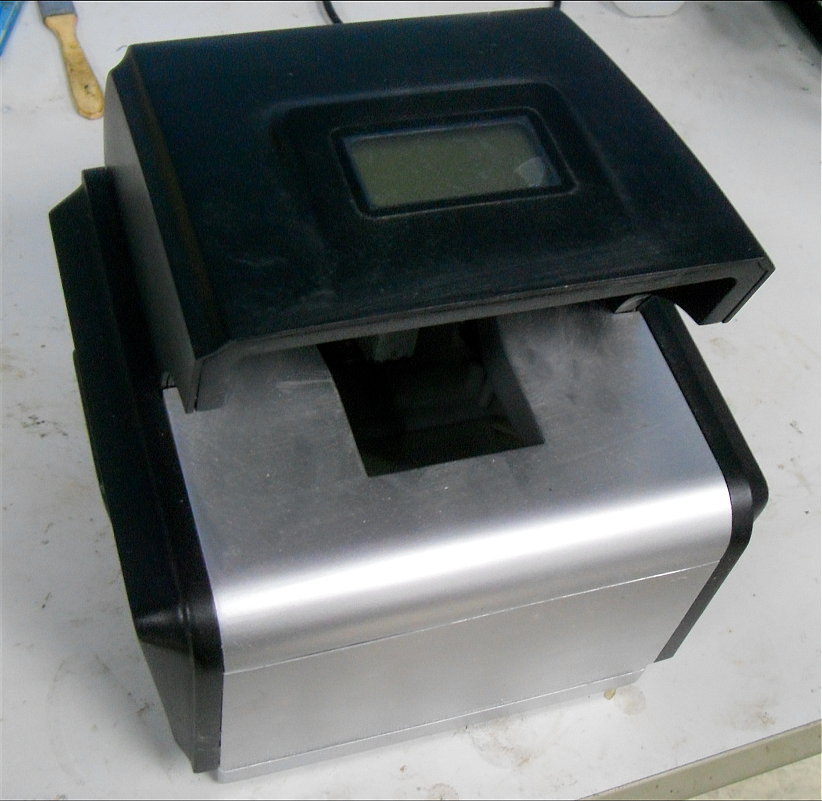
\includegraphics[width=\textwidth]{im/testim}
        \caption{Test Figure}
        \end{figure}
    \column{0.5\textwidth}
        \begin{figure}
        \centering
        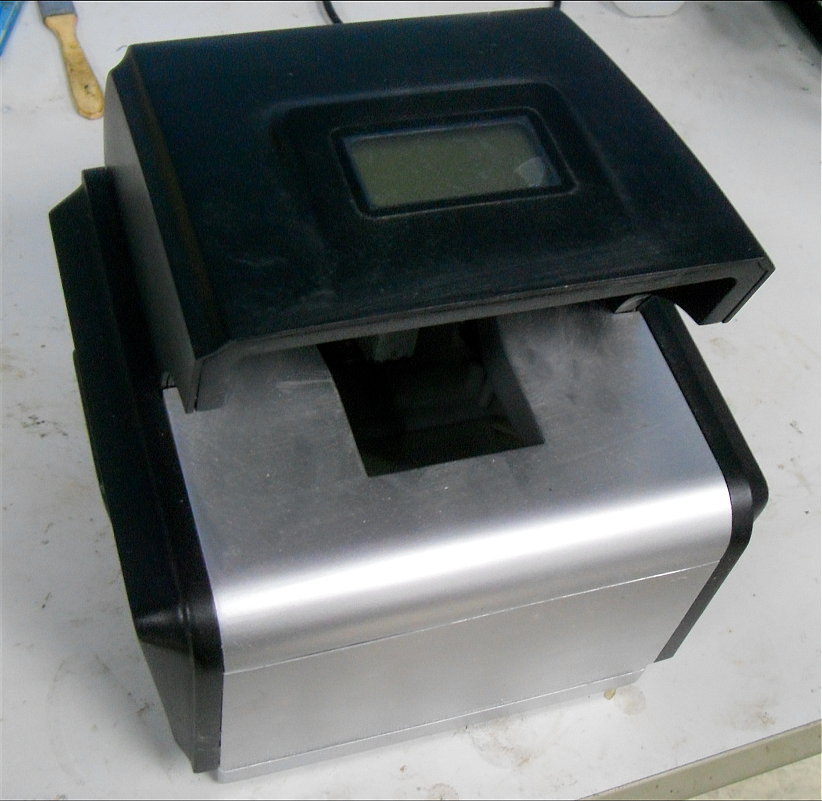
\includegraphics[width=\textwidth]{im/testim}
        \caption{Test Figure}
        \end{figure}
    \end{columns}
\end{frame}

\subsection{Image and Text}
\begin{frame}[t]{\subsecname} % t-top, c-center, s-shrank
    \begin{columns}
    \column{0.5\textwidth}
        \begin{figure}
        \centering
        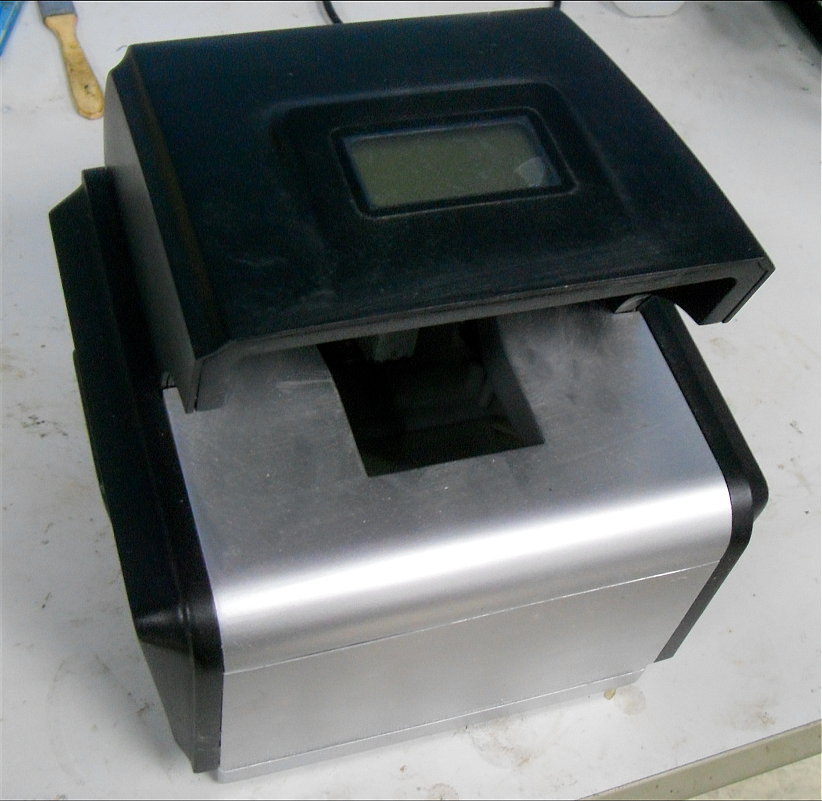
\includegraphics[width=\textwidth]{im/testim}
        \caption{Test Figure}
        \end{figure}
    \column{0.5\textwidth}
        Use the \texttt{columns} environment to display the image and text in the same frame side by side vertically.
    \end{columns}
\end{frame}

\begin{frame}[t]{\subsecname} % t-top, c-center, s-shrank
    \begin{columns}
    \column{0.5\textwidth}
        Use the \texttt{columns} environment to display the image and text in the same frame side by side vertically.
    \column{0.5\textwidth}
        \begin{figure}
        \centering
        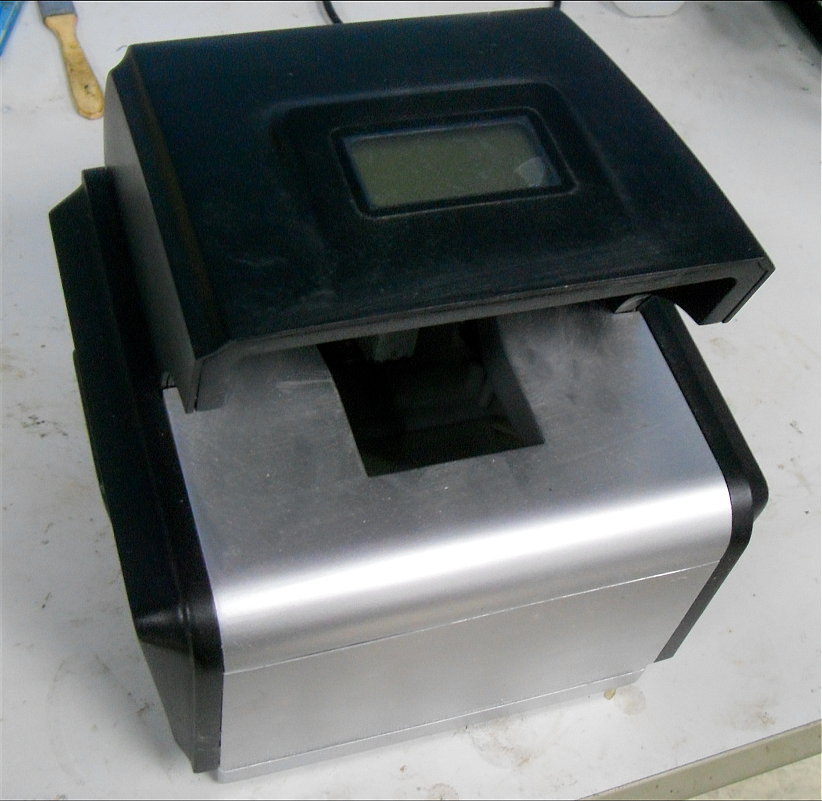
\includegraphics[width=\textwidth]{im/testim}
        \caption{Test Figure}
        \end{figure}
    \end{columns}
\end{frame}

\subsection{Don't be overcrowded}
\begin{frame}[t]{\subsecname} % t-top, c-center, s-shrank
    \begin{enumerate}
    \item Don't be overcrowded.
    \item Don't be overcrowded.
    \item Don't be overcrowded.
    \item Don't be overcrowded.
    \item Don't be overcrowded.

    \item Don't be overcrowded.
    \item Don't be overcrowded.
    \item Don't be overcrowded.
    \item Don't be overcrowded.
    \item Don't be overcrowded.
    
    \item Don't be overcrowded.
    \item Don't be overcrowded.
    \item Don't be overcrowded.
    \item Don't be overcrowded.
    \item Don't be overcrowded.
    
    \item Don't be overcrowded.
    \end{enumerate}
\end{frame}

\begin{frame}[shrink]{The \texttt{shrink}ed Frame} % t-top, c-center, shrink
    \begin{enumerate}
    \item \texttt{shrink} buys you a little space, but it is not recommended.
    \item Don't be overcrowded.
    \item Don't be overcrowded.
    \item Don't be overcrowded.
    \item Don't be overcrowded.

    \item Don't be overcrowded.
    \item Don't be overcrowded.
    \item Don't be overcrowded.
    \item Don't be overcrowded.
    \item Don't be overcrowded.
    
    \item Don't be overcrowded.
    \item Don't be overcrowded.
    \item Don't be overcrowded.
    \item Don't be overcrowded.
    \item Don't be overcrowded.
    
    \item Don't be overcrowded.
    \item Don't be overcrowded.
    \item Don't be overcrowded.
    \item Don't be overcrowded.
    \item Don't be overcrowded.
    \end{enumerate}
\end{frame}

\begin{frame}[allowframebreaks]{The \texttt{break}ed Frame} % t-top, c-center, shrink
    \begin{enumerate}
    \item \texttt{allowframebreaks} breaks a frame into several frames.
    \item Don't be overcrowded.
    \item Don't be overcrowded.
    \item Don't be overcrowded.
    \item Don't be overcrowded.

    \item Don't be overcrowded.
    \item Don't be overcrowded.
    \item Don't be overcrowded.
    \item Don't be overcrowded.
    \item Don't be overcrowded.
    
    \item Don't be overcrowded.
    \item Don't be overcrowded.
    \item Don't be overcrowded.
    \item Don't be overcrowded.
    \item Don't be overcrowded.
    
    \item Don't be overcrowded.
    \item Don't be overcrowded.
    \item Don't be overcrowded.
    \item Don't be overcrowded.
    \item Don't be overcrowded.
    \end{enumerate}
\end{frame}

%%%%%%%%%%%%%%%%%%%%%%%%%% Ending %%%%%%%%%%%%%%%%%%%%%%%%%%%%%%%%%%%%%%%%%%%%%%%%%%%%%%%%%%%%%

\begin{frame}<handout:0>[c]{Q \& A}
    \centerline{\LARGE{Any questions?\footnote{\texttt{<handout:0>} option removes this frame from \texttt{handout}.}}}    
\end{frame}    
    
\begin{frame}<handout:0>[c]{Acknowledgments}
    \centerline{\LARGE{Thank You For Your Attention!\footnote{Don't forget to Acknowledge.}}} 
\end{frame}
    
    
\end{document}



